\documentclass{ntuabeamer}

\usepackage[utf8]{inputenc}
\usepackage{amsmath}
\usepackage{amssymb}
\usepackage{graphicx}
\usepackage{booktabs}
\usepackage{appendixnumberbeamer}
\usepackage{tikz}
\usetikzlibrary{arrows.meta,calc,positioning}

\title{Recurrent Neural Networks}
\author{}
\date{}

\definecolor{courseblue}{HTML}{3F7CAC}
\definecolor{courseorange}{HTML}{D97706}
\definecolor{coursegreen}{HTML}{27864A}
\definecolor{coursegray}{HTML}{667085}
\definecolor{coursepurple}{HTML}{7656A3}
\definecolor{coursered}{HTML}{B5473C}
\definecolor{courselightblue}{HTML}{DCE9F5}
\definecolor{courselightorange}{HTML}{F9E4C8}

\tikzset{
  flow/.style={-{Latex[length=3mm]},very thick,courseblue},
  backflow/.style={-{Latex[length=3mm]},very thick,courseorange},
  box/.style={draw,rounded corners,very thick,align=center,minimum width=1.5cm,minimum height=0.9cm},
  state/.style={circle,draw,very thick,minimum size=0.85cm,inner sep=0pt}
}

\newcommand{\recap}[2]{%
  \begin{frame}{Recap: #1}
    \vfill
    \centering
    {\color{courseblue}\large\bfseries #2\par}
    \vfill
  \end{frame}%
}

\begin{document}

\begin{frame}[plain]
  \makepresentationtitle
\end{frame}

\begin{frame}{Roadmap}
  We ask how a network can read a sequence, why it is hard to train, and how gated cells help.
  \medskip
  \tableofcontents
\end{frame}

% ---------------------------------------------------------------- sequences and state

\section{Sequences and the Hidden State}
\sectiondivider{Sequences and the Hidden State}

\begin{frame}{A Sequence Has an Explicit Time Axis}
  \[
    \mathbf{X}\in\mathbb{R}^{B\times T\times d_x}
  \]
  \begin{itemize}
    \item $B$: number of sequences in a batch.
    \item $T$: number of time steps.
    \item $d_x$: features observed at each step.
  \end{itemize}
  \centering
  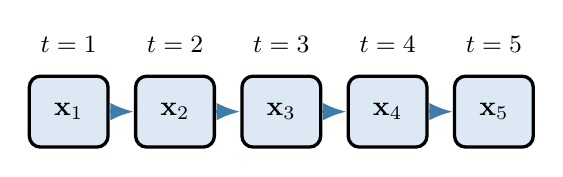
\begin{tikzpicture}[node distance=0.65cm]
    \foreach \t in {1,...,5}{
      \node[box,fill=courselightblue,minimum width=1.0cm] (x\t) at (1.35*\t,0) {$\mathbf{x}_{\t}$};
      \node[above=0.15cm of x\t,font=\small] {$t=\t$};
    }
    \foreach \t in {1,...,4}{
      \pgfmathtruncatemacro{\next}{\t+1}
      \draw[flow] (x\t) -- (x\next);
    }
  \end{tikzpicture}

  \vspace{0.1cm}
  Example: $B=32$ vibration recordings, each with $T=1000$ time steps and $d_x=3$ sensor channels.
  The order of the steps carries information.
\end{frame}

\begin{frame}{Why a Sequence Model Needs Memory}
  \begin{itemize}
    \item To predict the next word of ``the clouds are in the \dots'', the earlier words matter.
    \item The stress in a beam now depends on the whole loading history, not only on the load at this instant.
    \item A dense network with a fixed number of inputs cannot handle sequences of varying length, and it does not share what it learns across time steps.
  \end{itemize}
  A sequence model must carry a summary of what it has seen so far from one step to the next.
\end{frame}

\begin{frame}{A Hidden State Summarizes the Past}
  The network keeps a vector $\mathbf{h}_t$, the hidden state: a learned, compressed summary of the inputs up to time $t$.
  At each step it combines the new input with the previous summary.
  \begin{itemize}
    \item $\mathbf{h}_0$ is the starting summary (zeros, or learned).
    \item The summary need not keep every detail of the past, only what is useful for the task.
  \end{itemize}
  The hidden state is the network's running memory.
\end{frame}

\begin{frame}{The Recurrent Update}
  \[
    \boxed{
      \mathbf{h}_t
      =\phi\!\left(
        \mathbf{W}_{xh}\mathbf{x}_t
        +\mathbf{W}_{hh}\mathbf{h}_{t-1}
        +\mathbf{b}_h
      \right)
    },
    \qquad
    \widehat{\mathbf{y}}_t
    =g\!\left(\mathbf{W}_{hy}\mathbf{h}_t+\mathbf{b}_y\right)
  \]
  \begin{itemize}
    \item $\phi$ is the activation function (usually $\tanh$), as in the dense-network lecture.
    \item $\mathbf{W}_{xh}$ reads the input, $\mathbf{W}_{hh}$ reads the previous state, $\mathbf{W}_{hy}$ reads the state to produce the output.
    \item $g$ is the output function chosen by the task: identity for regression, softmax for classes.
  \end{itemize}
  The new state is a nonlinear mix of the current input and the old state.
\end{frame}

\begin{frame}{A Hidden State in Numbers}
  One-dimensional state: $h_t=\tanh(0.5\,x_t+0.8\,h_{t-1})$, with $h_0=0$ and the inputs $x_1=1$, $x_2=x_3=0$.
  \begin{center}
    \begin{tabular}{lccc}
      \toprule
      step $t$ & 1 & 2 & 3\\
      \midrule
      input $x_t$ & 1 & 0 & 0\\
      state $h_t$ & $0.46$ & $0.35$ & $0.28$\\
      \bottomrule
    \end{tabular}
  \end{center}
  The single input at $t=1$ is still visible in $h_3$, although no later input repeated it.
  The state remembers the past, and the memory fades with each step.
\end{frame}

\begin{frame}{Recurrence Feeds the State Back Into the Cell}
  \centering
  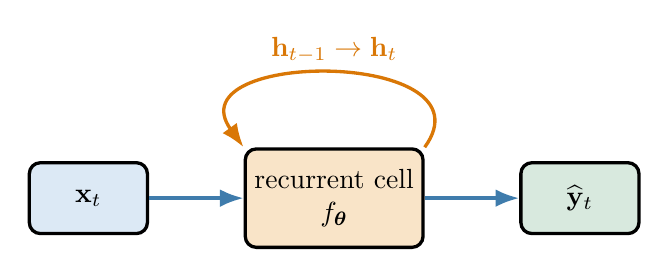
\begin{tikzpicture}[node distance=1.2cm]
    \node[box,fill=courselightorange,minimum width=2.2cm,minimum height=1.25cm] (cell) {recurrent cell\\$f_{\boldsymbol{\theta}}$};
    \node[box,fill=courselightblue,left=of cell] (input) {$\mathbf{x}_t$};
    \node[box,fill=coursegreen!18,right=of cell] (output) {$\widehat{\mathbf{y}}_t$};
    \draw[flow] (input) -- (cell);
    \draw[flow] (cell) -- (output);
    \draw[backflow]
      (cell.north east) .. controls +(0.9,1.25) and +(-0.9,1.25) ..
      node[above] {$\mathbf{h}_{t-1}\rightarrow\mathbf{h}_t$} (cell.north west);
  \end{tikzpicture}

  \vspace{0.2cm}
  The cell $f_{\boldsymbol\theta}$ (with parameters $\boldsymbol\theta$: all the $\mathbf W$ and $\mathbf b$ above) takes the input and the old state and returns the output and the new state.
  The loop sends the new state back as the next step's old state.
\end{frame}

\begin{frame}{Unrolling Reveals Shared Parameters Through Time}
  \centering
  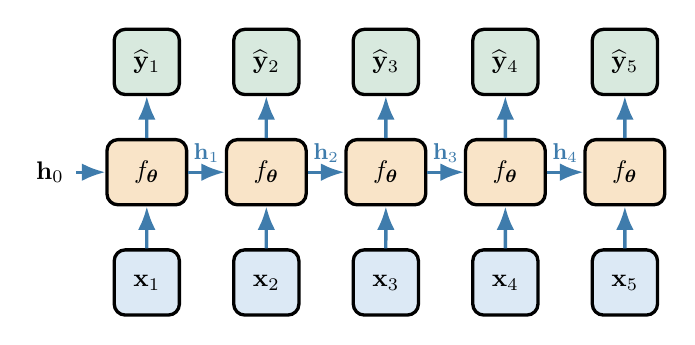
\begin{tikzpicture}[node distance=0.58cm,scale=0.92,transform shape]
    \foreach \t in {1,...,5}{
      \node[box,fill=courselightorange,minimum width=1.1cm] (h\t) at (1.65*\t,0) {$f_{\boldsymbol{\theta}}$};
      \node[box,fill=courselightblue,minimum width=0.9cm,below=of h\t] (x\t) {$\mathbf{x}_{\t}$};
      \node[box,fill=coursegreen!18,minimum width=0.9cm,above=of h\t] (y\t) {$\widehat{\mathbf{y}}_{\t}$};
      \draw[flow] (x\t) -- (h\t);
      \draw[flow] (h\t) -- (y\t);
    }
    \foreach \t in {1,...,4}{
      \pgfmathtruncatemacro{\next}{\t+1}
      \draw[flow] (h\t) -- node[above,font=\small] {$\mathbf{h}_{\t}$} (h\next);
    }
    \node[left=0.45cm of h1] {$\mathbf{h}_0$};
    \draw[flow] ($(h1.west)+(-0.4,0)$) -- (h1);
  \end{tikzpicture}

  \vspace{0.2cm}
  Unrolling draws one copy of the cell per time step: a deep network whose layers are the time steps.
  Every copy uses the same $\boldsymbol{\theta}$.
\end{frame}

\begin{frame}{Output Timing Depends on the Task}
  \centering
  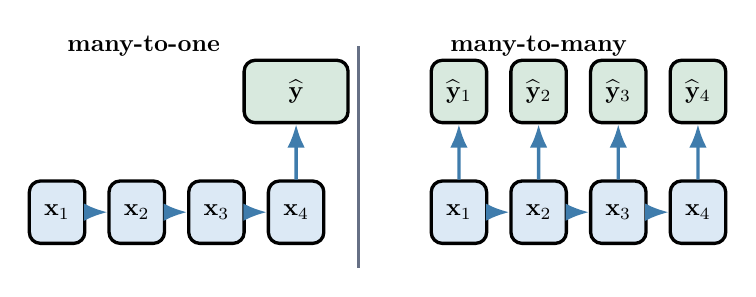
\begin{tikzpicture}[scale=0.88,transform shape]
    \node[font=\bfseries] at (2.4,2.4) {many-to-one};
    \foreach \t in {1,...,4}{
      \node[box,fill=courselightblue,minimum width=0.8cm] (a\t) at (1.15*\t,0) {$\mathbf{x}_{\t}$};
    }
    \foreach \t in {1,...,3}{
      \pgfmathtruncatemacro{\next}{\t+1}
      \draw[flow] (a\t) -- (a\next);
    }
    \node[box,fill=coursegreen!18,above=0.8cm of a4] (ao) {$\widehat{\mathbf{y}}$};
    \draw[flow] (a4) -- (ao);

    \draw[coursegray,very thick] (5.5,-0.8) -- (5.5,2.4);
    \node[font=\bfseries] at (8.1,2.4) {many-to-many};
    \foreach \t in {1,...,4}{
      \node[box,fill=courselightblue,minimum width=0.8cm] (b\t) at (5.8+1.15*\t,0) {$\mathbf{x}_{\t}$};
      \node[box,fill=coursegreen!18,minimum width=0.8cm,above=0.8cm of b\t] (bo\t) {$\widehat{\mathbf{y}}_{\t}$};
      \draw[flow] (b\t) -- (bo\t);
    }
    \foreach \t in {1,...,3}{
      \pgfmathtruncatemacro{\next}{\t+1}
      \draw[flow] (b\t) -- (b\next);
    }
  \end{tikzpicture}

  \vspace{0.1cm}
  Many-to-one: read the whole sequence, then answer once (for example, classify a recording).
  Many-to-many: produce an output at every step (for example, track a signal over time).
  The same cell serves both; only when we read the output changes.
\end{frame}

\recap{Sequences and the Hidden State}{A recurrent network carries a hidden state through time and reuses one cell at every step; next, how it is trained.}

% ---------------------------------------------------------------- training

\section{Training Through Time}
\sectiondivider{Training Through Time}

\begin{frame}{Backpropagation Also Unrolls Through Time}
  \centering
  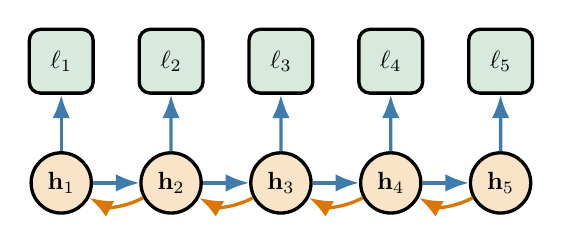
\begin{tikzpicture}[scale=0.9,transform shape]
    \foreach \t in {1,...,5}{
      \node[state,fill=courselightorange] (h\t) at (1.55*\t,0) {$\mathbf{h}_{\t}$};
      \node[box,fill=coursegreen!18,minimum width=0.9cm,above=0.8cm of h\t] (l\t) {$\ell_{\t}$};
      \draw[flow] (h\t) -- (l\t);
    }
    \foreach \t in {1,...,4}{
      \pgfmathtruncatemacro{\next}{\t+1}
      \draw[flow] (h\t) -- (h\next);
      \draw[backflow,bend left=28] (h\next) to (h\t);
    }
  \end{tikzpicture}
  \vspace{0.3cm}
  \[
    L=\sum_{t=1}^{T}\ell_t
  \]
  The total loss $L$ adds the loss $\ell_t$ of every step. Blue arrows: forward in time. Orange arrows: error signals flowing backward in time.
  Backpropagation through time (BPTT) is ordinary backpropagation on the unrolled network: each step's error reaches all earlier states.
\end{frame}

\begin{frame}{One Parameter, Many Uses}
  The unrolled network uses the same weights at every time step.
  \begin{itemize}
    \item The gradient of a weight is the sum of its gradient contributions from every time step.
    \item Each time step adds its own piece, so no special rule is needed beyond ordinary backpropagation.
  \end{itemize}
  Shared weights get one total gradient assembled from all time steps; the formula is in the appendix.
\end{frame}

\begin{frame}{Long Dependencies: Many Small Factors Multiply}
  To learn that an early input matters for a late output, the error signal must travel back through every step in between.
  At each step it is multiplied by a factor: the Jacobian $\mathbf J_k=\partial\mathbf h_k/\partial\mathbf h_{k-1}$,
  which says how strongly the previous state influences the next one.
  \[
    \frac{\partial\mathbf{h}_T}{\partial\mathbf{h}_t}
    =\mathbf{J}_T\mathbf{J}_{T-1}\cdots\mathbf{J}_{t+1}
  \]
  Intuition with one number per step: if every factor is $0.5$, then after $20$ steps the signal is
  $0.5^{20}\approx10^{-6}$; if every factor is $1.5$, it is $1.5^{20}\approx3300$.
  A long product shrinks to almost nothing or blows up, unless the factors stay close to one.
\end{frame}

\begin{frame}{Vanishing and Exploding Gradients}
  \centering
  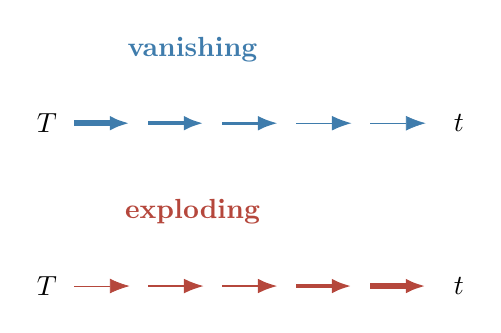
\begin{tikzpicture}[scale=0.94]
    \node[font=\bfseries,courseblue] at (2.5,2.4) {vanishing};
    \foreach \t/\size in {0/8,1/6,2/4,3/2,4/1}{
      \draw[-{Latex[length=2.5mm]},line width=\size*0.25pt,courseblue]
        (0.9+1.0*\t,1.4) -- ++(0.75,0);
    }
    \node[left] at (0.8,1.4) {$T$};
    \node[right] at (5.9,1.4) {$t$};

    \node[font=\bfseries,coursered] at (2.5,0.2) {exploding};
    \foreach \t/\size in {0/1,1/2,2/4,3/6,4/8}{
      \draw[-{Latex[length=2.5mm]},line width=\size*0.25pt,coursered]
        (0.9+1.0*\t,-0.8) -- ++(0.75,0);
    }
    \node[left] at (0.8,-0.8) {$T$};
    \node[right] at (5.9,-0.8) {$t$};
  \end{tikzpicture}

  \vspace{0.1cm}
  Arrow thickness shows the size of the error signal as it travels back from step $T$ to step $t$.
  For the simple recurrent cell above, $\mathbf J_k$ is the recurrent weight matrix times the activation slopes.
  Rough rule (intuition, not an exact law): factors below one make the signal vanish, above one make it explode.
  Either way, early inputs get little useful learning signal, so long dependencies are hard to learn.
\end{frame}

\begin{frame}{Gradient Clipping Limits Exploding Updates}
  \[
    \boxed{
      \widetilde{\mathbf{g}}
      =\begin{cases}
        \mathbf{g}, & \|\mathbf{g}\|_2\leq\tau,\\[2mm]
        \displaystyle\tau\frac{\mathbf{g}}{\|\mathbf{g}\|_2},
          & \|\mathbf{g}\|_2>\tau.
      \end{cases}
    }
  \]
  \begin{itemize}
    \item $\mathbf g$ is the gradient and $\tau>0$ is the clipping threshold: the largest gradient length we allow.
    \item Gradients shorter than $\tau$ are left unchanged.
    \item Longer gradients are rescaled to length $\tau$; their direction is kept.
  \end{itemize}
  Clipping prevents a single huge step; it does not fix vanishing gradients.
\end{frame}

\recap{Training Through Time}{Backpropagation through time works on the unrolled network, but long products of factors make gradients vanish or explode; next, a cell design that protects the memory.}

% ---------------------------------------------------------------- LSTM

\section{Gated Memory: LSTM and GRU}
\sectiondivider{Gated Memory: LSTM and GRU}

\begin{frame}{LSTM Adds an Explicit Memory Path}
  \centering
  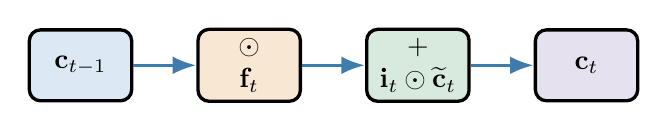
\begin{tikzpicture}[node distance=0.8cm]
    \node[box,fill=courselightblue,minimum width=1.3cm] (previous) {$\mathbf{c}_{t-1}$};
    \node[box,fill=courseorange!18,minimum width=1.3cm,right=of previous] (forget) {$\odot$\\$\mathbf{f}_t$};
    \node[box,fill=coursegreen!18,minimum width=1.3cm,right=of forget] (add) {$+$\\$\mathbf{i}_t\odot\widetilde{\mathbf{c}}_t$};
    \node[box,fill=coursepurple!18,minimum width=1.3cm,right=of add] (current) {$\mathbf{c}_t$};
    \draw[flow] (previous) -- (forget);
    \draw[flow] (forget) -- (add);
    \draw[flow] (add) -- (current);
  \end{tikzpicture}
  \vspace{0.3cm}
  \begin{itemize}
    \item A second state, the cell state $\mathbf c_t$, is the long-term memory. It is updated by scaling (forgetting) and adding, not by squashing it through an activation each step.
    \item Learned gates $\mathbf f_t$ (forget) and $\mathbf i_t$ (input) decide what to keep and what to write.
  \end{itemize}
  The additive path lets information and gradients travel many steps with little loss.
\end{frame}

\begin{frame}{LSTM Gates Read the Current Input and Previous State}
  Let $\mathbf{q}_t=[\mathbf{x}_t;\mathbf{h}_{t-1}]$ be the current input stacked on top of the previous state. Each gate is a small dense layer on $\mathbf q_t$ with a sigmoid, so its entries lie between $0$ (closed) and $1$ (open):
  \[
    \mathbf{f}_t=\sigma(\mathbf{W}_f\mathbf{q}_t+\mathbf{b}_f),
    \qquad
    \mathbf{i}_t=\sigma(\mathbf{W}_i\mathbf{q}_t+\mathbf{b}_i),
    \qquad
    \mathbf{o}_t=\sigma(\mathbf{W}_o\mathbf{q}_t+\mathbf{b}_o)
  \]
  \[
    \widetilde{\mathbf{c}}_t
    =\tanh(\mathbf{W}_c\mathbf{q}_t+\mathbf{b}_c)
  \]
  \begin{itemize}
    \item Forget gate $\mathbf{f}_t$: how much of the old memory to keep.
    \item Input gate $\mathbf{i}_t$: how much of the new candidate $\widetilde{\mathbf c}_t$ to write.
    \item Output gate $\mathbf{o}_t$: how much of the memory to reveal as the state.
  \end{itemize}
  The gates are learned soft switches that depend on the current input and the past.
\end{frame}

\begin{frame}{LSTM Updates Memory Before Exposing State}
  \[
    \boxed{
      \mathbf{c}_t
      =\mathbf{f}_t\odot\mathbf{c}_{t-1}
      +\mathbf{i}_t\odot\widetilde{\mathbf{c}}_t
    }
    \qquad
    \boxed{
      \mathbf{h}_t
      =\mathbf{o}_t\odot\tanh(\mathbf{c}_t)
    }
  \]
  \begin{itemize}
    \item $\odot$ multiplies two vectors entry by entry, so each gate scales each memory entry.
    \item The cell state $\mathbf{c}_t$ carries memory; the hidden state $\mathbf{h}_t$ is the exposed output.
  \end{itemize}
  The cell state is rewritten by gated forgetting plus gated writing.
\end{frame}

\begin{frame}{An LSTM Update in Numbers}
  Take one memory entry with $c_{t-1}=1$, forget gate $f_t=0.9$, input gate $i_t=0.5$, candidate $\widetilde c_t=0.4$:
  \[
    c_t=0.9\cdot1+0.5\cdot0.4=1.1 .
  \]
  \begin{itemize}
    \item With $f_t=0.9$ the old value is mostly kept; with $f_t=0$ it would be erased, and the entry would be $0.2$.
    \item Repeating with $f=0.9$, a stored value decays like $0.9^{20}\approx0.12$ after $20$ steps: far slower than the $0.5^{20}\approx10^{-6}$ earlier.
  \end{itemize}
  Gates near one keep memory; gates near zero erase it. LSTMs make long memory easier to learn, not guaranteed.
\end{frame}

\begin{frame}{GRU: A Lighter Gated Cell}
  The gated recurrent unit (GRU) keeps a single state and uses two gates instead of three, so it has fewer parameters.
  One gate decides how much of the old state to replace with a new candidate.
  \begin{itemize}
    \item It works in much the same way as the LSTM and is often a simpler alternative.
    \item The equations are in the appendix.
  \end{itemize}
  Both LSTM and GRU use learned gates to control what is remembered.
\end{frame}

\recap{Gated Memory}{Gated cells keep memory on an additive path and learn when to keep, write and reveal it; next, where recurrent models fit among alternatives.}

% ---------------------------------------------------------------- use

\section{When to Use Recurrent Models}
\sectiondivider{When to Use Recurrent Models}

\begin{frame}{Recurrence Is Sequential by Construction}
  \begin{itemize}
    \item State $\mathbf h_t$ cannot be computed before $\mathbf h_{t-1}$.
    \item Training can run many sequences in parallel, but not all time steps of one sequence.
    \item The state is a compact memory with fixed cost per step, so a model can process a stream as it arrives.
  \end{itemize}
  RNNs remain useful for online signals, control, and small stateful models.
\end{frame}

\begin{frame}{Attention Creates Direct Paths Between Time Steps}
  \centering
  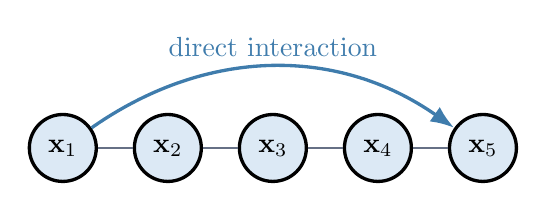
\begin{tikzpicture}[scale=0.92]
    \foreach \t in {1,...,5}{
      \node[state,fill=courselightblue] (x\t) at (1.45*\t,0) {$\mathbf{x}_{\t}$};
    }
    \foreach \t in {1,...,4}{
      \pgfmathtruncatemacro{\next}{\t+1}
      \draw[coursegray,thick] (x\t) -- (x\next);
    }
    \draw[flow,bend left=35] (x1) to node[above] {direct interaction} (x5);
  \end{tikzpicture}

  \vspace{0.2cm}
  In a recurrent model, step 1 reaches step 5 only through the states of steps 2, 3 and 4. Attention connects them directly.
  Transformers replace recurrence with attention (the next topic); for large offline datasets this is often preferable.
\end{frame}

\begin{frame}{Summary: Recurrent Models Share Computation Across Time}
  \begin{itemize}
    \item A hidden state summarizes the sequence so far, updated by one shared cell.
    \item Unrolling shows parameter sharing and the long gradient paths.
    \item Long products can make gradients vanish or explode; clipping limits the exploding case.
    \item LSTMs and GRUs add learned gates to protect memory.
    \item Attention is a different route to long-range interaction.
  \end{itemize}
  Recurrence suits streaming data; attention suits long-range links in large offline datasets.
\end{frame}

\appendix

\sectiondivider{Appendix: optional depth}

\begin{frame}{Shared Parameters Accumulate Gradients from Every Use}
  Write the state update as $\mathbf h_t=f_{\boldsymbol\theta}(\mathbf x_t,\mathbf h_{t-1})$.
  Let $\boldsymbol\delta_t=\mathrm dL/\mathrm d\mathbf h_t$ be the total error signal at $\mathbf h_t$
  after all later losses have been propagated backward. Then
  \[
    \frac{\mathrm d L}{\mathrm d\boldsymbol\theta}
    =\sum_{t=1}^{T}
      \boldsymbol\delta_t^{\mathsf T}
      \frac{\partial f_{\boldsymbol\theta}
      (\mathbf x_t,\mathbf h_{t-1})}{\partial\boldsymbol\theta}.
  \]
  \begin{itemize}
    \item Each local use of $\boldsymbol\theta$ contributes once.
    \item $\boldsymbol\delta_t$ includes the direct loss at step $t$ and all later losses.
  \end{itemize}
\end{frame}

\begin{frame}{The Recurrent Jacobian Bounds Gradient Scale}
  For $\mathbf h_t=\phi(\mathbf z_t)$ with $\mathbf z_t=\mathbf W_{xh}\mathbf x_t+\mathbf W_{hh}\mathbf h_{t-1}+\mathbf b_h$,
  \[
    \mathbf J_t
    =\operatorname{diag}(\phi'(\mathbf z_t))\mathbf W_{hh},
    \qquad
    \left\|\mathbf J_T\cdots\mathbf J_{t+1}\right\|_2
    \leq \prod_{k=t+1}^{T}\|\mathbf J_k\|_2.
  \]
  \begin{itemize}
    \item Norms uniformly below one imply the product contracts, so gradients vanish.
    \item Large norms permit growth; they do not guarantee it.
    \item $\mathbf J_t$ changes with the state and input, so this is an upper bound, not a prediction.
  \end{itemize}
\end{frame}

\begin{frame}{The Additive Cell Path Supports Gradient Flow}
  Holding the gates fixed for the local derivative,
  \[
    \frac{\partial\mathbf c_t}{\partial\mathbf c_{t-1}}
    =\operatorname{diag}(\mathbf f_t).
  \]
  Across several steps, the direct cell-state path contains
  \[
    \prod_{k=t+1}^{T}\operatorname{diag}(\mathbf f_k).
  \]
  Forget gates near one preserve information and gradients; gates near zero erase them on purpose.
  LSTMs mitigate but do not eliminate long-horizon difficulties.
\end{frame}

\begin{frame}{GRU Equations}
  \[
    \mathbf{u}_t=\sigma(\mathbf{W}_u[\mathbf{x}_t;\mathbf{h}_{t-1}]+\mathbf{b}_u),
    \qquad
    \mathbf{r}_t=\sigma(\mathbf{W}_r[\mathbf{x}_t;\mathbf{h}_{t-1}]+\mathbf{b}_r)
  \]
  \[
    \widetilde{\mathbf{h}}_t
    =\tanh\!\left(\mathbf{W}_h
      [\mathbf{x}_t;\mathbf{r}_t\odot\mathbf{h}_{t-1}]+\mathbf{b}_h\right)
  \]
  \[
    \boxed{
      \mathbf{h}_t
      =(1-\mathbf{u}_t)\odot\mathbf{h}_{t-1}
      +\mathbf{u}_t\odot\widetilde{\mathbf{h}}_t
    }
  \]
  The update gate $\mathbf u_t$ blends old state and candidate; the reset gate $\mathbf r_t$ decides how much old state the candidate sees.
  Here $\mathbf u_t=1$ selects the candidate; some references reverse the two coefficients.
\end{frame}

\begin{frame}{Truncated BPTT Limits the Reverse-Time Horizon}
  Split a long stream into windows of $K$ steps. Carry the hidden state forward, but stop its gradient at each window boundary.
  \[
    \frac{\partial\mathbf h_t}{\partial\mathbf h_{t-K}}
    \quad\text{is omitted when the boundary is detached.}
  \]
  \begin{itemize}
    \item Memory and reverse-pass cost are bounded by $K$.
    \item Dependencies longer than $K$ receive no direct gradient credit through that boundary.
  \end{itemize}
\end{frame}

\begin{frame}{Bidirectional RNNs Use Past and Future Context}
  \[
    \overrightarrow{\mathbf h}_t
      =f_\rightarrow(\mathbf x_t,\overrightarrow{\mathbf h}_{t-1}),
    \qquad
    \overleftarrow{\mathbf h}_t
      =f_\leftarrow(\mathbf x_t,\overleftarrow{\mathbf h}_{t+1}),
    \qquad
    \mathbf h_t=[\overrightarrow{\mathbf h}_t;\overleftarrow{\mathbf h}_t].
  \]
  Two cells read the sequence in opposite directions and their states are concatenated.
  This improves offline sequence labeling when the whole sequence is available.
  It is invalid for causal streaming predictions that must not access future inputs.
\end{frame}

\begin{frame}{Autoregressive Decoders Feed Outputs Back as Inputs}
  \[
    p(\mathbf y_{1:T}\mid\mathbf x)
    =\prod_{t=1}^{T}p(\mathbf y_t\mid\mathbf y_{<t},\mathbf x).
  \]
  During teacher forcing, training conditions on the observed previous target $\mathbf y_{t-1}$.
  At inference, the model conditions on its own previous prediction $\widehat{\mathbf y}_{t-1}$.
  This mismatch can compound errors over long generated sequences.
\end{frame}

\end{document}
